\documentclass{beamer}
\usepackage{inconsolata}
\usepackage{caption}
\usepackage{color}
\usepackage{listings}
\usepackage{subfig}
\usepackage{cooltooltips}
\usepackage{hyperref}
\usepackage{perpage}
\usepackage[normalem]{ulem}
\setbeamertemplate{navigation symbols}{}%remove navigation symbols
\usepackage{listings}
\usepackage{color}
\usepackage{framed}

\definecolor{background}{RGB}{39, 40, 34}
\definecolor{string}{RGB}{230, 219, 116}
\definecolor{comment}{RGB}{117, 113, 94}
\definecolor{normal}{RGB}{248, 248, 242}
\definecolor{identifier}{RGB}{166, 226, 46}



\lstset{
  language=C,               			% choose the language of the code
  alsolanguage=Python,            			% choose the language of the code
  alsolanguage=Java,            			% choose the language of the code
  numbers=none,                   		% where to put the line-numbers
  stepnumber=1,                   		% the step between two line-numbers.        
  numbersep=5pt,                  		% how far the line-numbers are from the code
  extendedchars=true,
  numberstyle=\tiny\color{black}\ttfamily,
  backgroundcolor=\color{background},  		% choose the background color. You must add \usepackage{color}
  showspaces=false,               		% show spaces adding particular underscores
  showstringspaces=false,         		% underline spaces within strings
  showtabs=false,                 		% show tabs within strings adding particular underscores
  frame=single,
  framerule=0pt,
  tabsize=4,                      		% sets default tabsize to 2 spaces
  captionpos=n,                   		% sets the caption-position to bottom
  breaklines=true,                		% sets automatic line breaking
  breakatwhitespace=true,         		% sets if automatic breaks should only happen at whitespace
  title=\lstname,                 		% show the filename of files included with \lstinputlisting;
  basicstyle=\color{normal}\tiny\ttfamily,					% sets font style for the code
  keywordstyle=\color{magenta}\tiny\ttfamily,	% sets color for keywords
  stringstyle=\color{string}\tiny\ttfamily,		% sets color for strings
  commentstyle=\color{comment}\tiny\ttfamily,	% sets color for comments
  emph={True, False, format_string, eff_ana_bf, permute, eff_ana_btr, KeyError,
  ValueError, ZeroDivisionError},
  emphstyle=\color{identifier}\tiny\ttfamily,
  morekeywords={with, as}
}

\lstset{literate=%
   *{0}{{{\color{cyan}0}}}1
    {1}{{{\color{cyan}1}}}1
    {2}{{{\color{cyan}2}}}1
    {3}{{{\color{cyan}3}}}1
    {4}{{{\color{cyan}4}}}1
    {5}{{{\color{cyan}5}}}1
    {6}{{{\color{cyan}6}}}1
    {7}{{{\color{cyan}7}}}1
    {8}{{{\color{cyan}8}}}1
    {9}{{{\color{cyan}9}}}1
}



\newenvironment{enum}{
\begin{enumerate}
  \setlength{\itemsep}{1pt}
  \setlength{\parskip}{0pt}
  \setlength{\parsep}{0pt}
}{\end{enumerate}}

\hypersetup{
  colorlinks=true,
  urlcolor=pink,
}

\MakePerPage{footnote}

\title{Python 101}
\subtitle{Lec06 \\ Classes}
\author{thoum}

\begin{document}
\frame{\titlepage}

\begin{frame}
\frametitle{Programming up till now}
Procedure-Oriented Programming\\
We pass values to functions, get values, pass them to another function....
  \begin{center}
  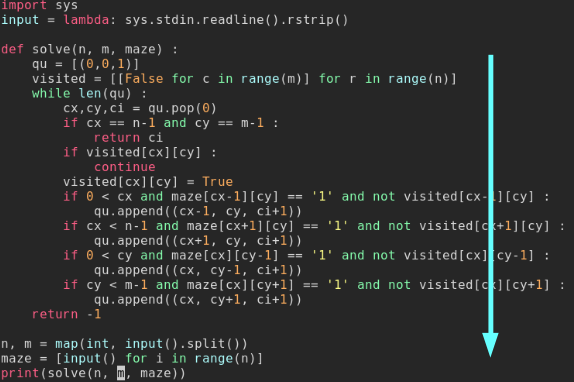
\includegraphics[width=80mm]{./code.png}
  \end{center}
\end{frame}

\begin{frame}
\frametitle{Procedure Oriented Programming}
  When programs get large, Procedure-Oriented might be \textit{too}
  complicated.\\
\end{frame}

\begin{frame}
\frametitle{Object Oriented Programming}
  Combine data and functionality in to an \textit{object}.\\
  View programs as object communicating with each other.
\end{frame}

\begin{frame}{Objects}
  Integers are objects (of the int class).

  Strings are objects (of the str class).

  $[1,2,3].sort()$ are their class methods\\
  $len([1,2,3])$ returns their internal data: length
\end{frame}

\begin{frame}
\frametitle{Creating Classes of our own}
  We don't usually use classes so much unless we start writing bigger programs.

  We are going to build a basis for a simple RPG game.
\end{frame}

\begin{frame}{The Basis}
  There are two characters in this game(for now).

  The boss, and you.

  They are both \textit{being}s(there are other \textit{being}s like the halflings,
  dragons, darkelves...).
\end{frame}

\begin{frame}{Beings}
  This becomes the basis(or the \textit{superclass, parentclass}) of all living things that freely
  roam the grounds of the middle earth.  Every \textit{being} can be
  characterized by a name, HP, MP, and their race.
\end{frame}

\begin{frame}{Beings code}
  \begin{lstinputlisting}[firstline=1, lastline=23]
    {./being.py}
  \end{lstinputlisting}
\end{frame}

\begin{frame}{Explanation}
  Names of classes begin with capital letters. (Just a convention, but follow
  it.)
  \begin{lstinputlisting}[firstline=1, lastline=1]
    {./being.py}
  \end{lstinputlisting}
\end{frame}

\begin{frame}{Explanation}
  We annotate classes and functions with triple quotes.
  \begin{lstinputlisting}[firstline=1, lastline=2]
    {./being.py}
  \end{lstinputlisting}
\end{frame}

\begin{frame}{Explanation}
  Class Variables are shared by all instances of the class.
  We will see in detail later.
  \begin{lstinputlisting}[firstline=1, lastline=5]
    {./being.py}
  \end{lstinputlisting}
\end{frame}


\begin{frame}{Explanation}
  Methods whose names are surrounded by 2 underscores
  (\textit{\_\_XXX\_\_}) are
  \textit{internal} methods.
  They are not meant to be called by the user; they are
  automatically called based on varying situations.
  \begin{lstinputlisting}[firstline=1, lastline=7]
    {./being.py}
  \end{lstinputlisting}
\end{frame}

\begin{frame}{Explanation}
  \textit{\_\_init\_\_()} is automatically called upon the creation of an object of the
  class.
  \begin{lstinputlisting}[firstline=7, lastline=14]
    {./being.py}
  \end{lstinputlisting}
\end{frame}

\begin{frame}{Explanation}
  Class methods are same as the functions we have learned, but for one
  \textbf{difference}. They need an extra argument at the beginning of the
  parameter list.\\\textit{But} we \textbf{do not} pass a value for this parameter when we
  \textbf{use} it. The parameter is used to indicate \textit{itself}, hence the
  \textit{\textbf{self}}.(Just a convention, but follow it.)
  \begin{lstinputlisting}[firstline=5, lastline=8]
    {./being.py}
  \end{lstinputlisting}
\end{frame}

\begin{frame}{Explanation}
  The fields(object variables) are created by \_\_init\_\_.\\
  \begin{lstinputlisting}[firstline=7, lastline=12]
    {./being.py}
  \end{lstinputlisting}
\end{frame}

\begin{frame}{Explanation}
  To see how we use class/object variables, see the $die(self)$
  method.\footnote{note the $self$!}\\
  This is used when a battle arises (remember, we were pretending to make an RPG game).
  \begin{lstinputlisting}[firstline=17, lastline=19]
    {./being.py}
  \end{lstinputlisting}
\end{frame}

\begin{frame}{Explanation}
  Just like how we use $self$ to access object variables, we can access Class
  Variables by their class name (Here, $Being$).\\
  Note that when an object changes its $class$ variable, other objects also see
  the change.\\($Class$ variables are not unique to the object).
  \begin{lstinputlisting}[firstline=20, lastline=22]
    {./being.py}
  \end{lstinputlisting}
\end{frame}


\begin{frame}{Using Classes}
  We usually put Class definitions in different files, but for the sake of
  simplicity, lets do it in the same file.\\
  We create an object of a class like the following.
  \begin{lstinputlisting}[firstline=25, lastline=27]
    {./being.py}
  \end{lstinputlisting}
\end{frame}

\begin{frame}{Using Classes}
  Two things to note
  \begin{enumerate}
    \item We didn't call $\_\_init\_\_$.
    \item We didn't add $self$.
  \end{enumerate}
  \begin{lstinputlisting}[firstline=25, lastline=25]
    {./being.py}
  \end{lstinputlisting}
\end{frame}

\begin{frame}{Using Classes}
  We can explicitly use the names of the parameters, for better understanding of the
  code.\footnote{We can actually do this with all functions.}
  \begin{lstinputlisting}[firstline=26, lastline=27]
    {./being.py}
  \end{lstinputlisting}
\end{frame}

\begin{frame}{The Dragon Slayer}
  We call an object's method like the following. Familiar?
  \begin{lstinputlisting}[firstline=29, lastline=29]
    {./being.py}
  \end{lstinputlisting}
\end{frame}

\begin{frame}{Practice}
  Type and Try
\end{frame}

\begin{frame}[fragile]{Overriding Internal Functions}
  \begin{lstlisting}
print((1,2,3)): (1, 2, 3)\\
print([1,2,3]): [1, 2, 3]\\
print(3): 3\\
print(boss): ?\\
print(you): ?
  \end{lstlisting}
\end{frame}

\begin{frame}{Overriding Internal Functions}
  To control how $print$ prints a class, we can fill in\\
  $\_\_repr\_\_$\\
  The return value has to be of type $string$, and the return value is what is printed.
\end{frame}

\begin{frame}{Practice}
  In our $Being$ Class, define the $\_\_repr\_\_$, so that printing an object
  of $Being$ Class prints its name, and race.
  ($i.e.$ "This being is a Dragon, of name Smaug")
\end{frame}

\begin{frame}{Combat}
  Now we implement combat for Beings.
  The combat method gets another $Being$, decrease its hp by $3$, and if its hp
  is less or equal than zero, make it die.
\end{frame}

\begin{frame}
\frametitle{Inheritance}
One usage of classes is Inheritance.
\end{frame}

\begin{frame}
\frametitle{Inheritance}
The child inherits every thing about its parent, and $+\alpha$.
\end{frame}

\begin{frame}[fragile]
\frametitle{Inheritance}
\begin{lstinputlisting}
  {./mylist.py}
\end{lstinputlisting}
\end{frame}

\begin{frame}{Explained}
  $MyList(list)$ means that this class will inherit from $list$.
  \begin{lstinputlisting}[firstline=1, lastline=1]
  {./mylist.py}
\end{lstinputlisting}
\end{frame}

\begin{frame}{Explained}
  The $super()$ returns the parent class. We use super() to access the parent
  classes data methods etc. Here, we initiate the parent first so that
  parameters are automatically filled in.
  \begin{lstinputlisting}[firstline=1, lastline=4]
  {./mylist.py}
\end{lstinputlisting}
\end{frame}

\begin{frame}{Explained}
  $min(lst), max(lst)$ takes time proprotional to N.\\
  Here, we keep track of min and max so that it can be known regardless of
  size.\\
  (Of course, there is no free lunch, there is extra cost of comparing at append.)
  \begin{lstinputlisting}[firstline=1, lastline=6]
  {./mylist.py}
  \end{lstinputlisting}
\end{frame}

\begin{frame}{Explained}
  Here, we override the parent's \_\_len\_\_, which determines the value
  returned when we do $len(lst)$.
  \begin{lstinputlisting}[firstline=7, lastline=9]
    {./mylist.py}
  \end{lstinputlisting}
\end{frame}

\begin{frame}{Explained}
  We override the append() of list, so that we keep track of \_min and \_max.\\
  After updating \_min and \_max, we insert to the list via super() call.
  \begin{lstinputlisting}[firstline=11, lastline=16]
    {./mylist.py}
  \end{lstinputlisting}
\end{frame}

\begin{frame}{Question}
  Are we done implementing MyList so that it correctlys keep track of min and max?
\end{frame}

\begin{frame}{Question}
  \begin{center}
    NO
  \end{center}
\end{frame}

\begin{frame}{The Catch}
  Everything that can be done to a $list$ can be done to a $MyList$.\\
  $pop(),\ del,\ insert(),\ mylst[3]=4,\ mylst[3:4]$... you name it.\\
  \mbox{}\\
  This means that to correctly keep track of min \& max, we have to override
  \textit{every single} method of a list that is capable of changing its
  contents.\\
  \mbox{}\\
  Can you remember all of them?
\end{frame}

\begin{frame}{Composition over Inheritance\footnote{Look this up in Google}}
    So, it is often wise to compose your class with a list, rather than inheriting
    it.
\end{frame}

\begin{frame}{MyList Composition Ver.}
  We can control the methods we provide for interaction with the internal list.
  \begin{lstinputlisting}[firstline=1, lastline=23]
    {./composition.py}
  \end{lstinputlisting}
\end{frame}

\begin{frame}{Inheritance?}
  We might use inheritance when the child has to provide every method its parents
  provide + $\alpha$. \\($i.e.$ The Gun class that inherits the Weapon class in an RPG
  game?). \\But Design Patterns are a complicated subject by itself, so we won't
  deal it in detail.
\end{frame}

\end{document}
